\chapter{The Compact Muon Solenoid Experiment at the Large Hadron Collider}
\graphicspath{{cms/figures/}{cms/}}

The Compact Muon Solenoid (CMS) experiment is one of the four experiments operating at the Large Hadron Collider (LHC) particle accelerator at the European Center for Nuclear Research (CERN), in the suburbs of Geneva, Switzerland. 
Along with ATLAS, LHCb and ALICE, they are the latest generation of high energy physics experiments to take place at high energy hadron colliders. 
CMS and ATLAS are multi-purpose experiments, looking for different types of processes arising from the proton-proton collisions at the LHC, while LHCb and ALICE are designed for specific purposes: rare processes involving flavor physics and QCD at high temperatures, respectively.  
In the following sections, the LHC will be briefly summarized, followed by a description of the CMS experiment.

\section{The LHC Accelerator Complex}

The Large Hadron Collider (LHC) is a circular proton-proton collider operated at European Organization for Nuclear Research (CERN) in Geneva, Switzerland \cite{LHC}. 
The collider has a circumference of 27 km and is located in the underground tunnel that hosted the Large Electron Positron (LEP) collider, operated from 1989 until 2000. 
The LHC ring includes two adjacent beam pipes, each containing one of two colliding beams, which travel in opposite directions. 
The two beams are focused and bent in their circular trajectory by a system of more than 1600 superconducting magnets: 
1232 dipole magnets operating at a temperature of less than 2 K generate a magnetic field of 8.3 T that maintains the circular motion of the two beams around the LHC; 
392 quadrupole magnets are used to keep the beams focused as they travel inside the collider. 
The main part of the LHC physics program consists in operating the machine as a proton-proton (pp) collider, while part of the machine schedule is periodically dedicated to the delivery of heavy-ion collisions. 

In the LHC, beams are accelerated by the electromagnetic field generated by radio-frequency cavities (eight per beam) located along the collider ring. 
Each of these cavities also operates in superconducting state, at a temperature of approximately 4.5 K, and can deliver a voltage of 2 MV at a frequency of 400 MHz. 
Prior to their injection in the LHC, the colliding particles are grouped together in bunches and pre-accelerated in a chained system of smaller accelerators, which complete the CERN accelerator complex. 
A layout of the CERN accelerator complex can be seen in Figure \ref{fig:lhc}.

\begin{figure*}[h]
\centering 
\includegraphics[width=0.99\textwidth]{figures/lhc}\hfil
\caption{Sketch of the CERN accelerator complex, including the Large Hadron Collider. }
\label{fig:lhc}
\end{figure*}

The LHC was designed to deliver pp collisions at a center of mass energy of $\sqrt{s} = 14$ TeV with an instantaneous luminosity of $10^{34}$ cm$^{-2}$s$^{-1}$, using a bunch-spacing of 25 ns (time period between two consecutive bunch crossings). 
In the first years of data-taking, the LHC operated below the design values to reduce the time needed for commissioning the machine and to follow a safer strategy concerning the operation of the LHC magnets.
The first run of the LHC physics program with pp collisions started in 2009 at $\sqrt{s} = 7$ TeV and continued through 2010 and 2011 reaching a maximum instantaneous luminosity of $3.5 \times 10^{33}$ cm$^{-2}$s$^{-1}$ with a bunch spacing of 50 ns, translated into 5 fb$^{-1}$ collected by the CMS experiment. 
During 2012 and 2013, the center of mass energy was increased to $\sqrt{s} = 8$ TeV, and the machine reached a peak instantaneous luminosity of $7.7 \times 10^{33}$ cm$^{-2}$s$^{-1}$. 
In this period the CMS experiment recorded a total integrated luminosity of 19.7 fb$^{-1}$ with all subdetectors fully operational and nominal magnetic field.

From 2013 to 2015, the LHC went through upgrades amed at operating the collider at its nominal configuration. 
The first stable collisions in 2015 were in May, at $\sqrt{s} = 13$ TeV, with a bunch spacing of 50 ns, then changed to 25 ns later in the year, reaching a peak luminosity of $5 \times 10^{33}$ cm$^{-2}$s$^{-1}$. 
By the end of the first year of the LHC Run-2, the CMS experiment recorded a total integrated
luminosity of 2.6 fb$^{-1}$ with a magnetic field of 3.8 T and all subdetectors in full operation. 
The year of 2016 was a record breaking period for the LHC, with a peak luminosity of $1.4\times10^{34}$ cm$^{-2}$s$^{-1}$ (reaching its nominal value) and an integrated luminosity of about 40 fb$^{-1}$ in ATLAS and CMS at $\sqrt{s} = 13$ TeV. 

\section{The CMS Experiment}

The CMS experiment is one of the multi-purpose experiments at the LHC \cite{cms_tdr}. 
Its goal is to measure both Standard Model processes and search for physics beyond the Standard Model. 
In order to achieve this, it must precisely reconstruct objects that are typically present at high energy colliders (photons, electrons, muons and hadronic jets), including their positions and 4-momenta (3-dimensional momentum plus energy).  

The overall CMS design is that of a cylindrical onion, meaning that every individual subdetector (specializing in measuring different types of event information) is stacked together concentrically, like onion layers. 
These different subdetectors are shown in Figure \ref{fig:cms_sketch}, and will be described in the following sections. 

In order to measure charged particles momenta with the desired precision, a strong magnetic field must be present at the experiment, so the momentum can be extracted from the particles' bending. 
The CMS magnet is a superconducting solenoid located between the CMS calorimeters and muon detectors. 
It is 13 meters long, with 6 meters of inner diameter, and provides a 3.8T magnetic field. 
With this geometry, the direction of the magnetic field will be different at the CMS tracker system, in which charged particles trajectories are measured close to the interaction point, and at the CMS muon system, which is a tracking subdetector specialized in measuring muon trajectories. 
This optimizes the muon momentum measurement by having two magnetic bendings in the reconstructed muon path, instead of only one. 

\begin{figure*}[h]
\centering 
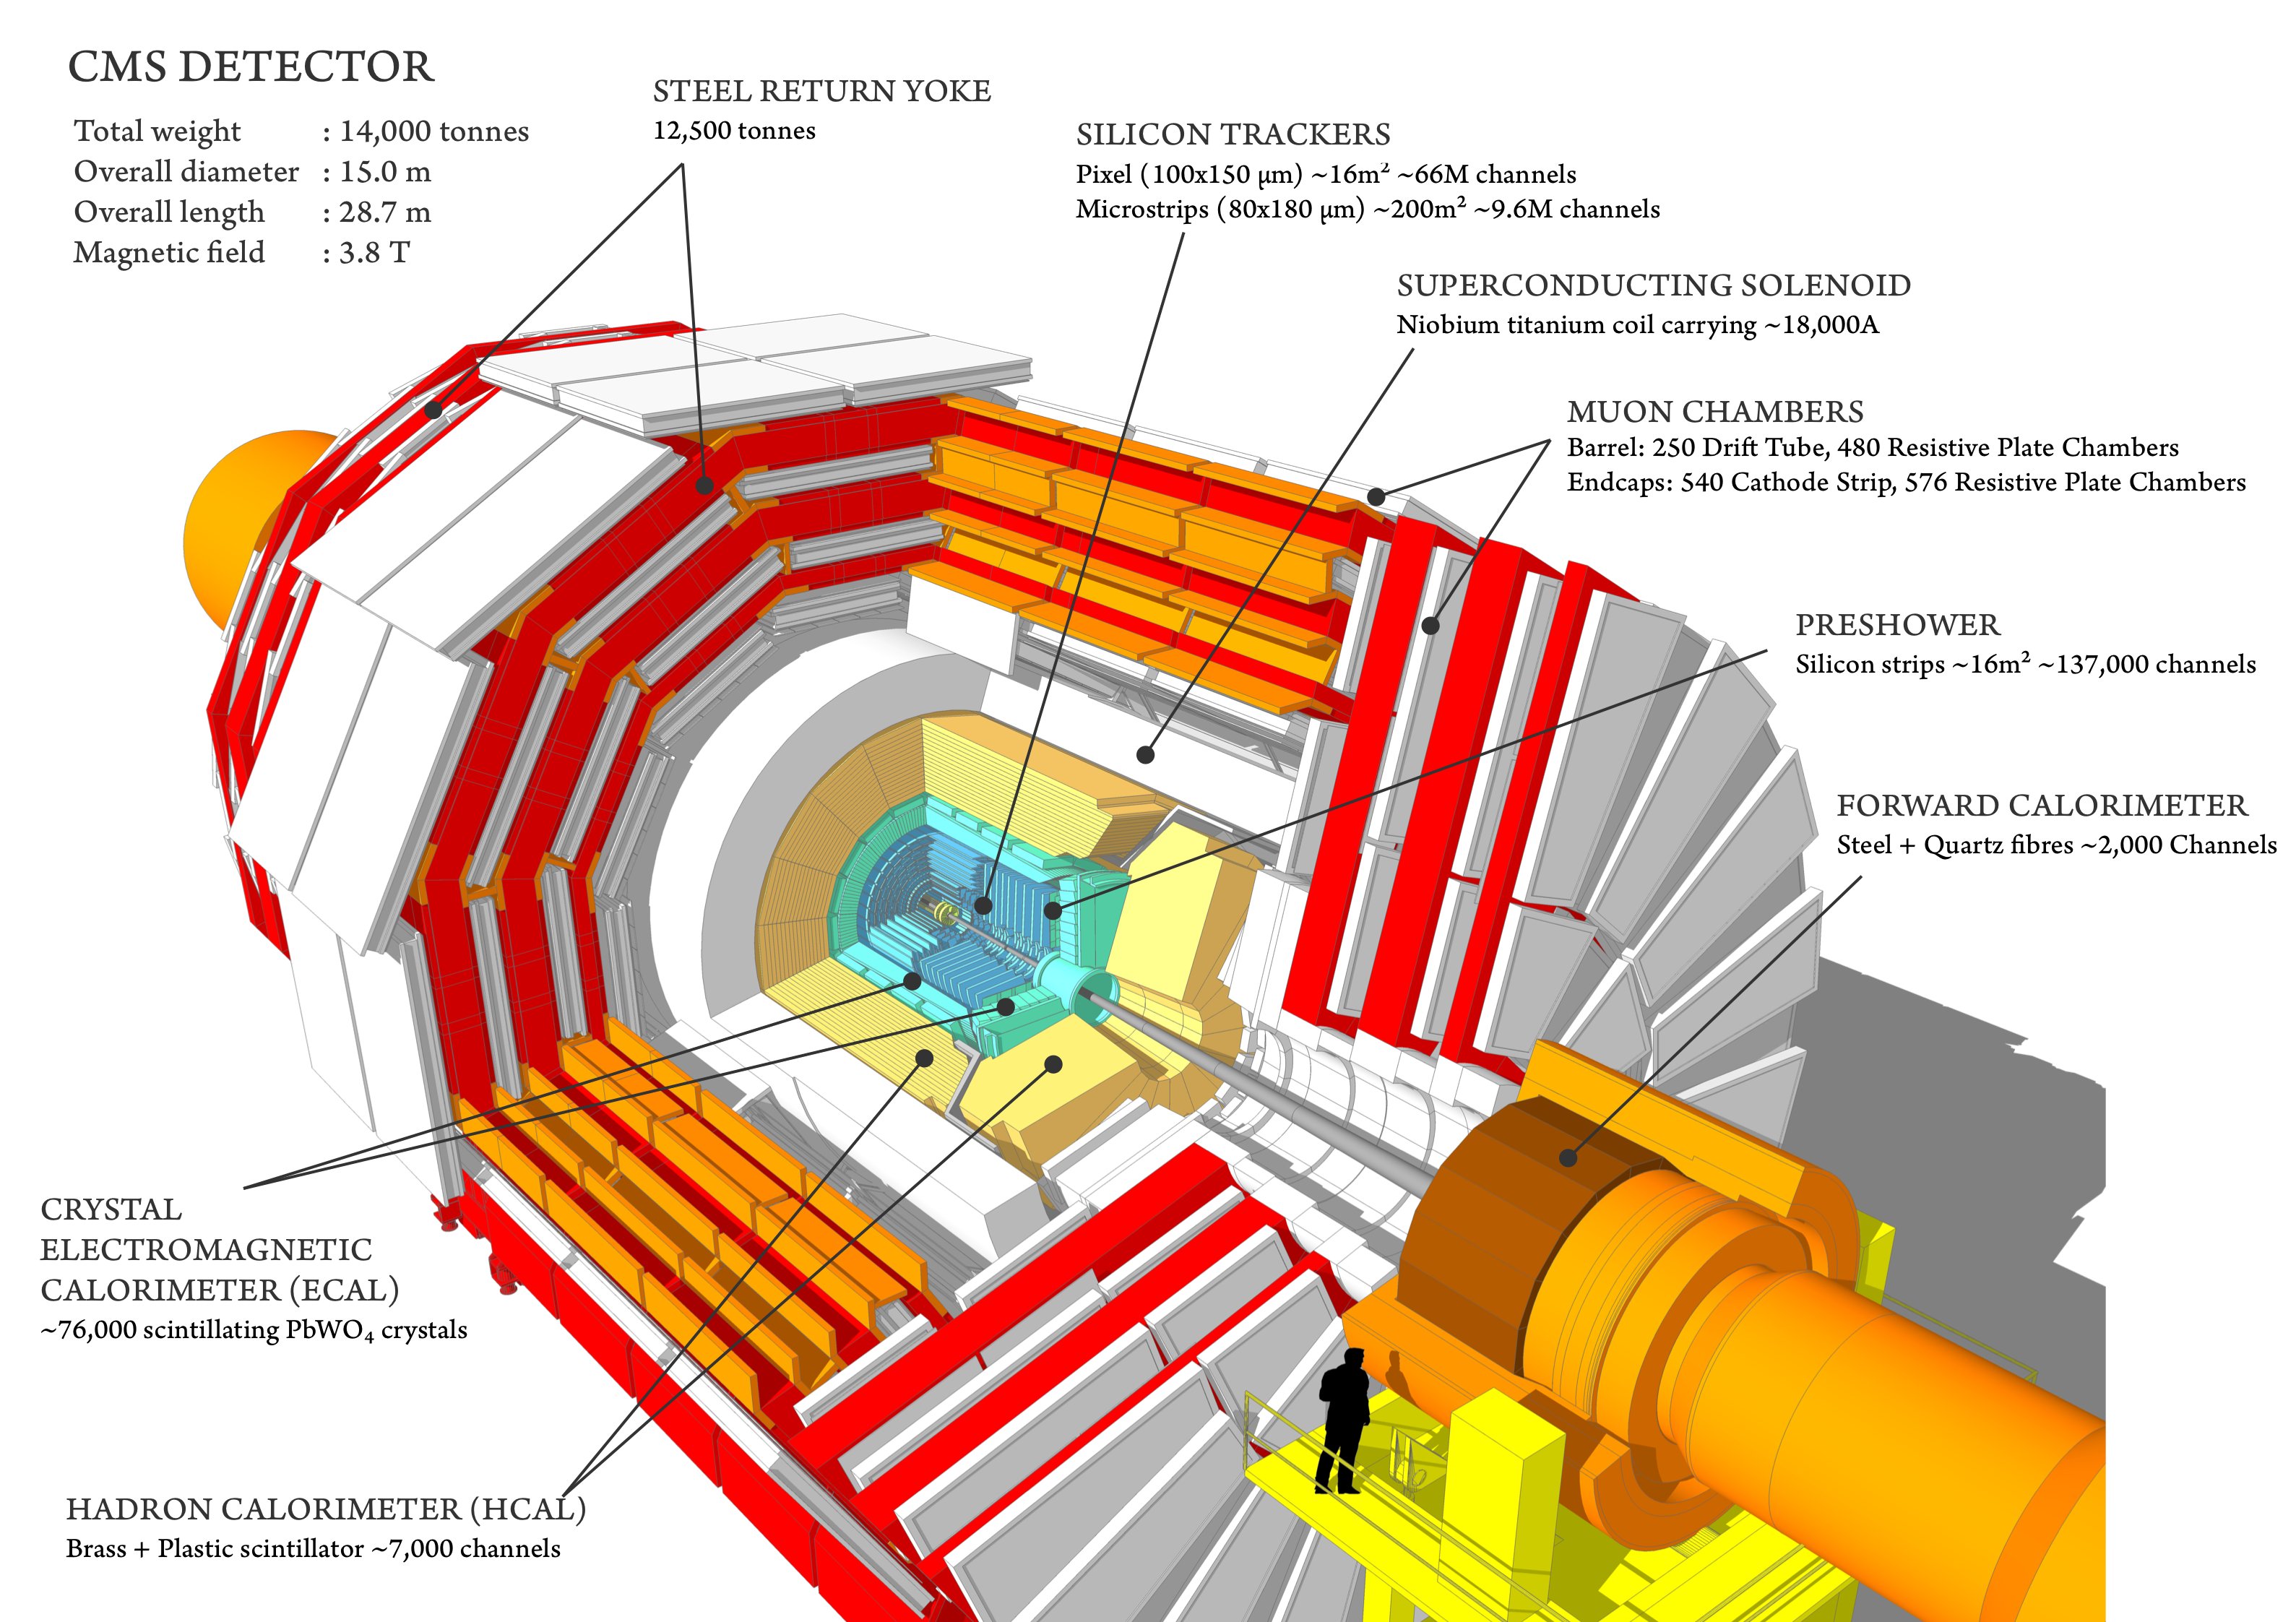
\includegraphics[width=0.99\textwidth]{figures/cms_sketch}\hfil
\caption{Sketch of the CMS experiment at the LHC, showing its different subdetectors stacked concentrically, like a cylindrical onion. }
\label{fig:cms_sketch}
\end{figure*}

Muons are long-lived particles that interact only via the electromagnetic and weak interactions. 
Differently from most of the particles produced at high energy collisions, they are able to go through all layers of CMS. 
Electrons, on the other hand, are stopped by the CMS Electromagnetic Calorimeter (ECAL), where they produce a particle shower based mostly on bremsstrahlung radiation (at high energies), and lose their energies almost completely. 
Due to the muons higher mass, they do not emit bremsstrahlung radiation as much as an electron, and therefore, are able to go through the CMS ECAL. 
Photons are measured by the ECAL in a similar way, the difference being that a photon shower starts by an electron-positron pair production from the original high energy photon. 
Muons also go through the CMS Hadronic Calorimeter (HCAL), which measures the energy of hadronic particles in a similar way that the ECAL measures the energy of photons and electrons, but with showers caused by the strong interaction. 

The CMS calorimeters are usually called destructive detectors, since, in order to measure the particle's energy, the particle must not leave the detector.
On the other hand, the tracking system aims to measure the particles' energy with little interaction to minimize the energy loss (so that it can be precisely measured by the calorimeters). This is performed, for example, through ionizing radiation on semi-conductor or gaseous devices. 

\subsection{The CMS Tracking Detectors}

The CMS tracking system must provide precise reconstruction for charged particles' trajectories with minimal interference in the particles' energies. 
These trajectories are reconstructed in terms of tracks, which are built from the different interactions of the incoming particle with the tracking system (hits). 
It must also cope with the high charged particle flux at various radii at high luminosity, which requires a high detector segmentation to reconstruct large track multiplicities at the same time. 

The CMS tracking system is entirely constructed of silicon, which detects hits by measuring electron-hole currents in the device produced by ionizing radiation. 
The geometry of these silicon sensors is different for three regions within the CMS detector, which are defined based on the charged particle flux from the LHC:

\begin{itemize}
\item  Closest to the interaction vertex where the particle flux is the highest, pixel detectors are placed. The size of a pixel is $\approx 100~\times~150 ~\mu$m$^{2}$, giving an occupancy of about 10$^{-4}$ hits per pixel sensor per LHC crossing.
\item In the intermediate region ($20 < r < 55$ cm), the particle flux is low enough to enable the usage of silicon microstrip detectors with a minimum cell size of $10$ cm $\times~80~\mu$m, leading to an occupancy of $\approx 2-3\%$ per LHC crossing.
\item In the outermost region ($r > 55$ cm) of the inner tracker, the particle flux has dropped sufficiently to allow use of larger-pitch silicon microstrips with a maximum cell size of $25$ cm $\times~180~\mu$m, while keeping the occupancy to $\approx 1\%$.
\end{itemize}

The pixel layers of the CMS tracker consist of three cylindrical layers of pixel modules surrounding the interaction point at radii of 4.4, 7.3 and 10.2 cm, and are topped at each side with two pixel module disks at $|z|$ = 34.5 cm and 46.5 cm. 
In total, it covers about 1 m$^{2}$, with 66 million pixels. 
The pixel detector delivers three high precision hits for each charged particle trajectory: the spatial resolution is measured to be about 10 $\mu$m for the $r-\phi$ measurement and about 20 $\mu$m for the $z$ measurement

After the pixels, the strip tracker detector covers the radial range between 20 cm and 116 cm. 
It consists of three different subsystems: the tracker inner barrel, inner disks and outer barrel (TIB, TID and TOB). 
The inner subsystems (TIB and TID) extend in radius from 20 cm to 55 cm, are composed of 4 layers in the barrel and 3 layers at each end, and deliver up to 4 measurements in $r-\phi$ by track, with a single hit resolution between 23 $\mu$m and 35 $\mu$m. 
The outer system (TOB) extends to a radius of 1.2m and to $|z| = 118$ cm, consists of 6 layers of micro-strip sensors, providing another 6 $r-\phi$ measurements with single point resolution between 35 $\mu$m and 53 $\mu$m. 

\begin{figure*}[h]
\centering 
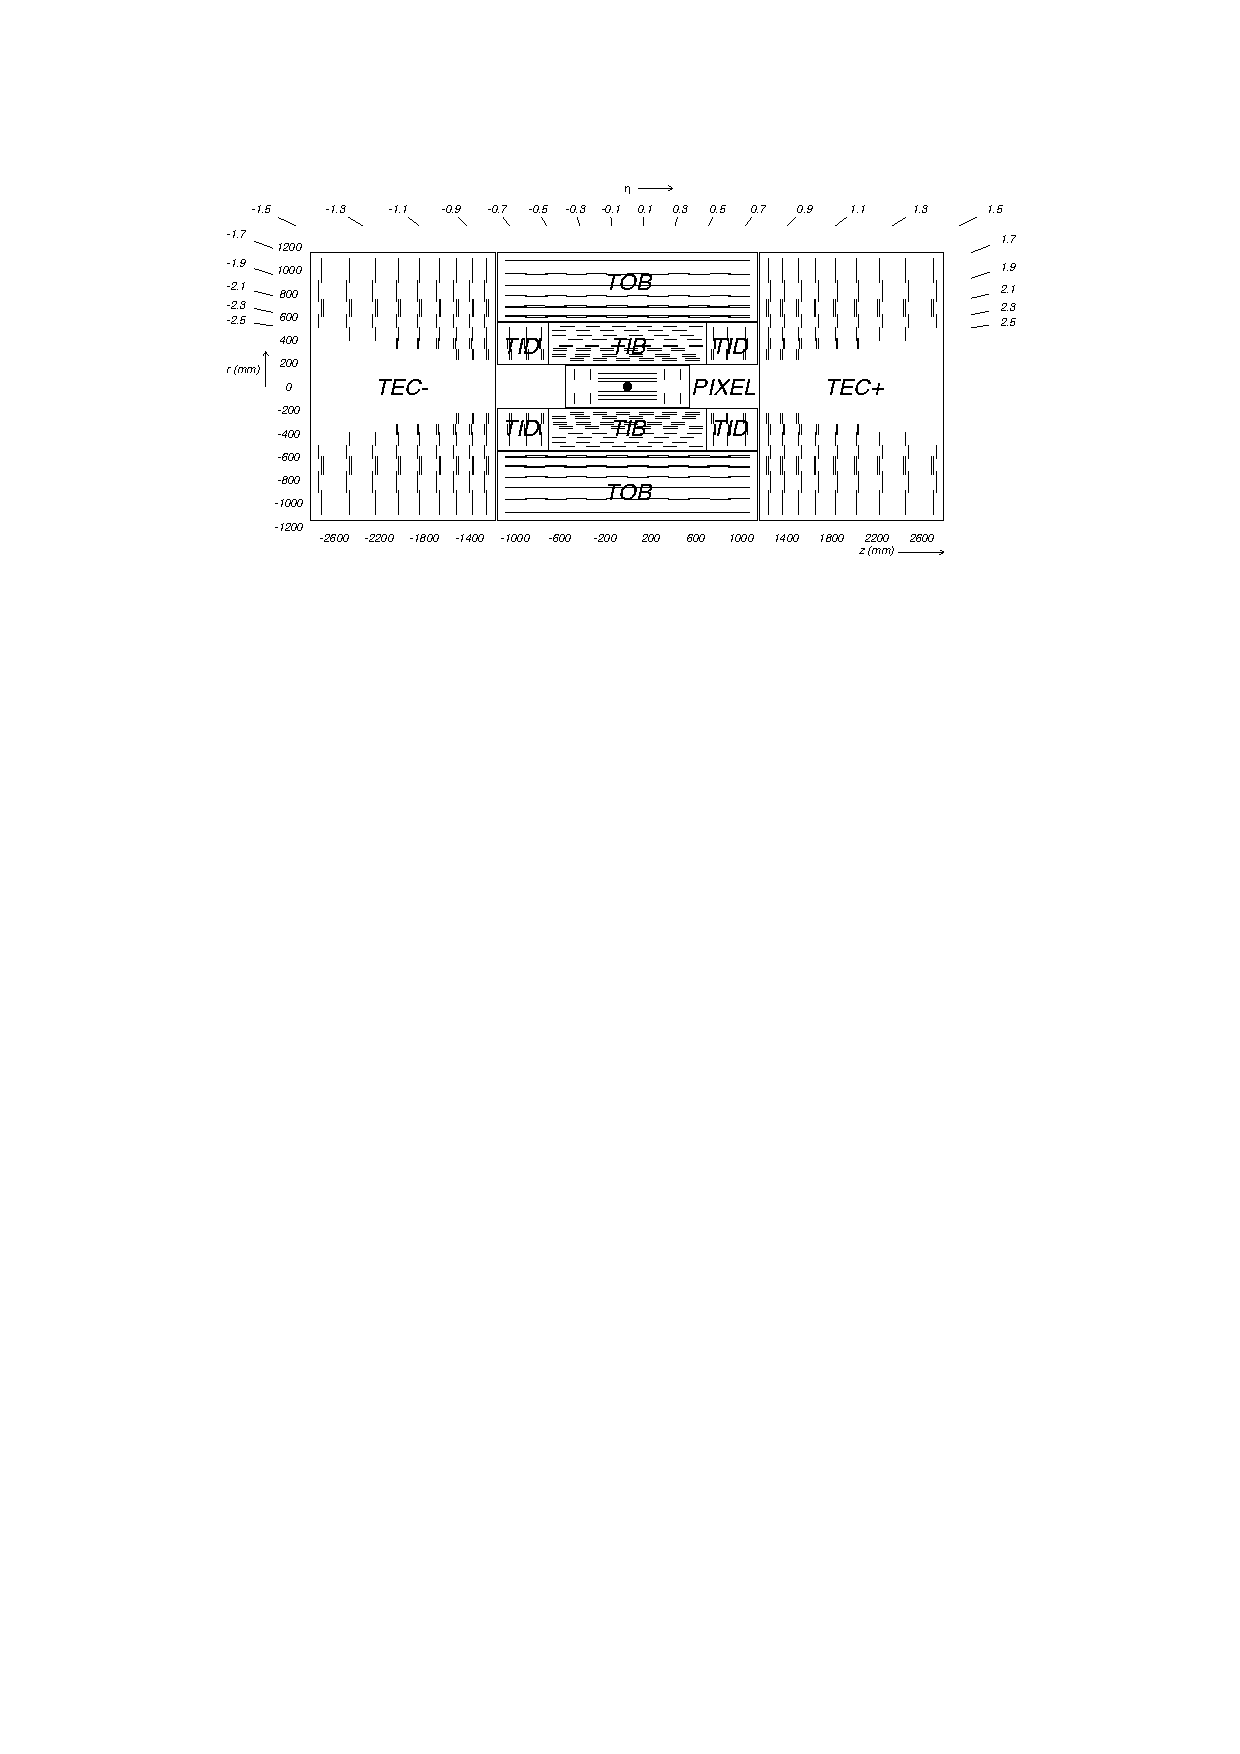
\includegraphics[width=0.99\textwidth]{figures/cms_tracker}\hfil
\caption{Sketch of the CMS tracker system. }
\label{fig:cms_tracker}
\end{figure*}


Beyond the TOB, the tracker endcaps (TEC+ and TEC-, where the sign relates to the location along the z axis) cover the region 124 cm $< |z| < $282 cm and 22.5 cm $< |r| <$ 113.5 cm. 
Each endcap consists of 9 disks, each with up to 7 rings of silicon micro-strips, providing up to 9 $r-\phi$ measurements per track. 
Additionally, some of the modules on the TIB, TID, TOB and TEC also carry a second micro-strip sensor module, mounted with a stereo angle of 100 mrad, to prove a measurement of the second coordinate (z in the barrel and r on the disks/endcaps). 
The overall CMS tracker module structure can be seen in Figure \ref{fig:cms_tracker}.


\subsection{The CMS Calorimetry Detectors}

The CMS calorimetry system consists of an electromagnetic calorimeter (ECAL), that measures the energies of electrons and photons, and a hadronic calorimeter (HCAL), that measures the energies of hadrons. 
The CMS HCAL will be described below, while the ECAL will be described in detail in Section \ref{sec_ecal}.

\subsubsection{The Hadronic Calorimeter}

The strong interaction forces quarks and gluons to hadronize, a process in which hadrons (particles consisting of quarks) are produced copiously from an initial colored particle. 
Some of these hadrons are unstable and can further decay into stable particles (such as leptons and other stable hadrons). 
At the end of the hadronization process, a quark/gluon is seen by CMS as a cluster of mostly electrons (with photons from bremsstrahlung), muons, pions, kaons, protons and neutrons, which are combined to form an object called a jet. 
Therefore, for precise jet measurements, the CMS experiments must precisely measure the energy of hadrons within a jet shower. 

The HCAL is limited by the ECAL in its inner radius, and by the CMS solenoid in its outer radius. 
In order to provide hermeticity and full coverage of the hadronic shower development, it must maximize the amount of absorber material in its region. 
This absorber material is a dense material with a high atomic number that causes the hadrons within a jet to further decay into less energetic particles.
The energy of these further decays are then measured by an active medium. 

The CMS HCAL is divided into three sections, the barrel (HB), the outer barrel region just outside the CMS solenoid (HO), the endcaps (HE) and the forward region closer to the beam pipe (HF), which can be seen in Figure \ref{fig:cms_hcal}. 
The HB and HE consist of brass absorbers, as it has a reasonably short interaction length, is easy to machine and is non-magnetic, while the active medium consists of plastic scintillator tiles read out with embedded wavelength-shifting (WLS) fibres. 
The HO functions as a tail catcher and it consists of only a layer of active medium of plastic scintillator tiles. 
The HF uses steel as absorber  and quartz fibers as active medium, a choice that is better suited for the more congested environment closer to the beam pipe. 
The photodetection readout is based on multi-channel hybrid photodiodes (HPDs) for HB, HE and HO, and on photomultiplier tubes (PMT) for HF.

\begin{figure*}[h]
\centering 
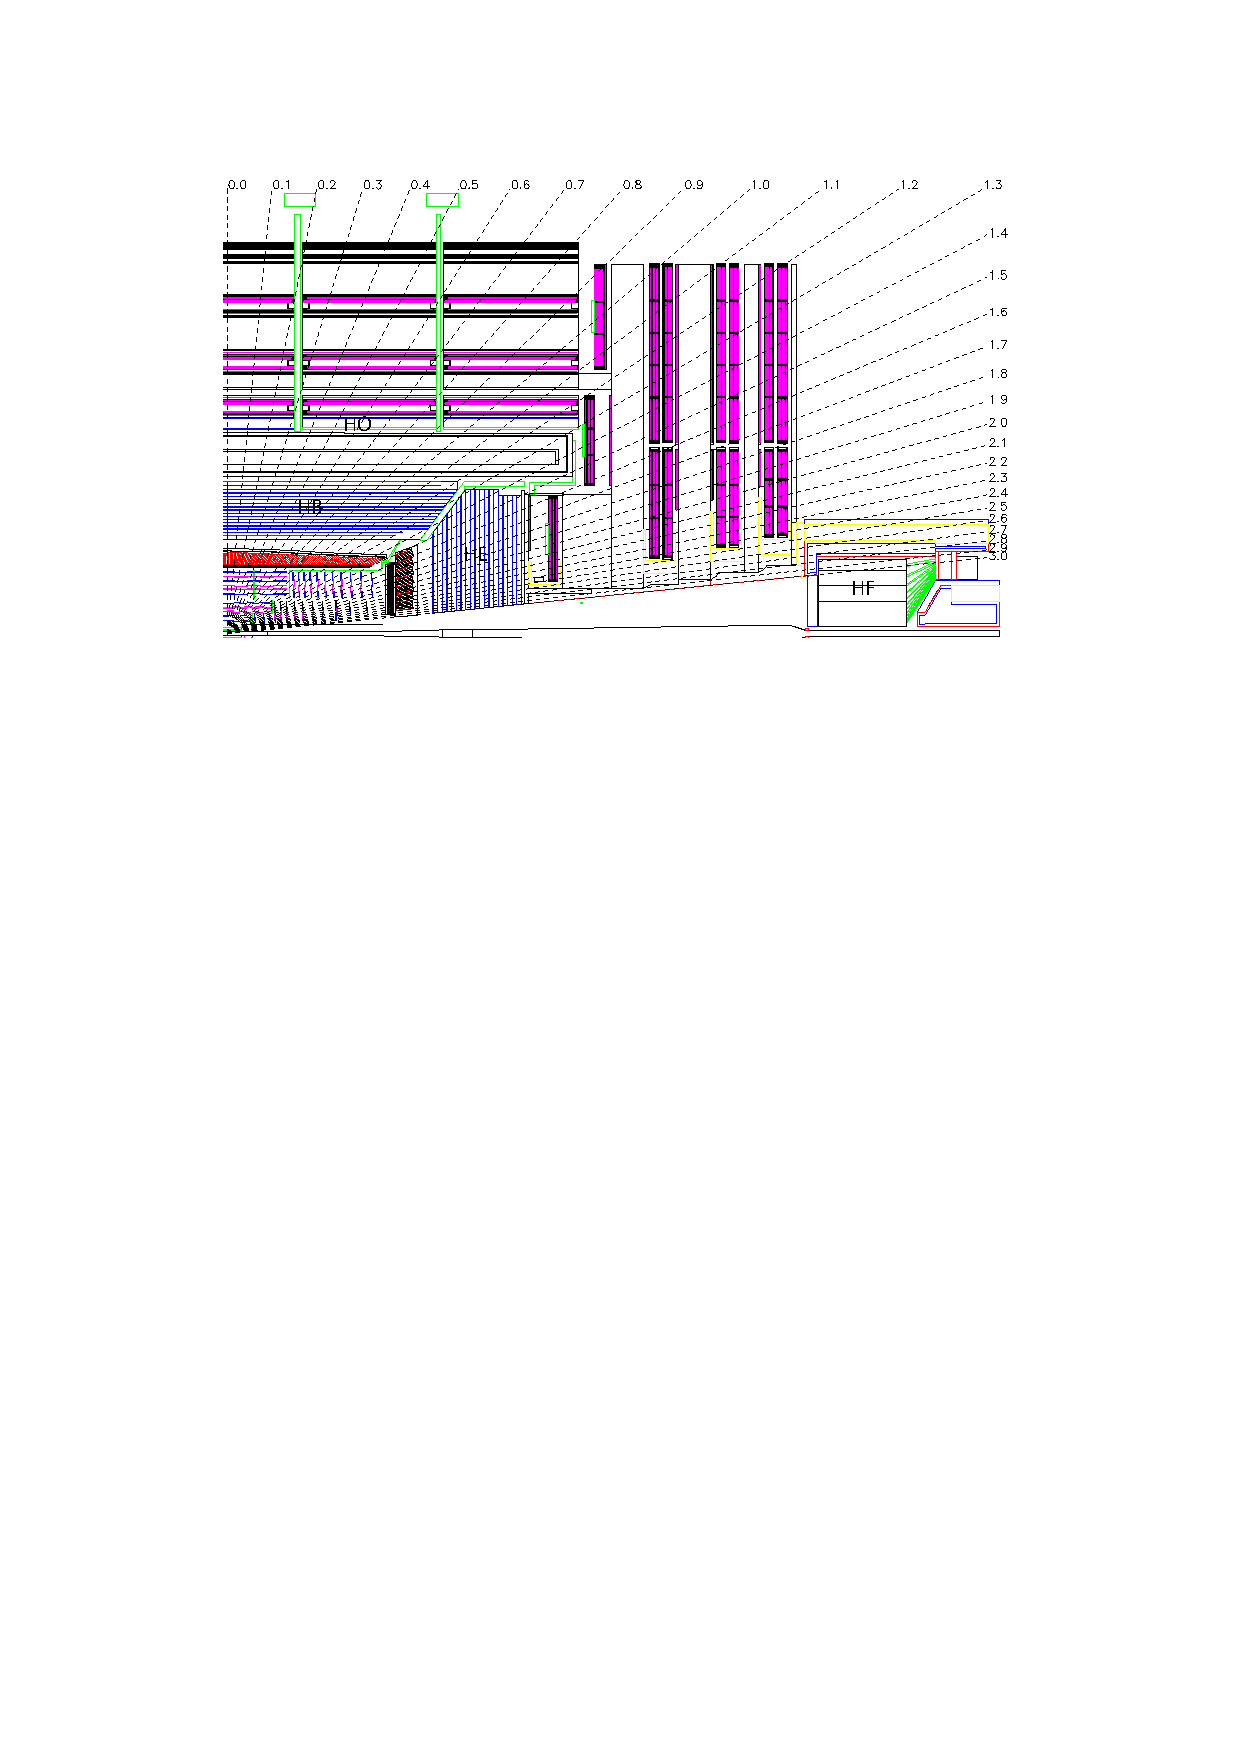
\includegraphics[width=0.99\textwidth]{figures/cms_hcal}\hfil
\caption{Sketch of the CMS hadronic calorimeter. }
\label{fig:cms_hcal}
\end{figure*}


The HB geometry consists of 32 towers covering the pseudorapidity region $-1.4 < \eta < 1.4$, resulting in 2304 towers with a segmentation $\Delta\eta\times\Delta\phi = 0.087\times0.087$.
Each HCAL endcap consists of 14 $\eta$ towers with $5^{o}$ $\phi$ segmentation, covering the pseudorapidity region $1.3 < |\eta| < 3.0$. 
For the 5 outermost towers (at smaller $\eta$) the $\phi$ segmentation is $5^{o}$ and the $\eta$ segmentation is 0.087. For the 8 innermost towers the $\phi$ segmentation is $10^{o}$, while the $\eta$ segmentation varies from 0.09 to 0.35 at the highest $\eta$. The total number of HE towers is 2304.
The HO detector contains scintillators with a thickness of 10 mm, which line the outside of the outer vacuum tank of the solenoid and cover the region $-1.26 < \eta < 1.26$. The tiles are grouped in $30^{o}$-sectors, matching the $\phi$ segmentation of the muon chambers to which it is attached. 
Coverage between pseudorapidities of $3.0 < |\eta| < 5.0$ is provided by the HF calorimeter. 
There are 13 HF towers in $\eta$, all with a size given by $\Delta\eta\approx0.175$, except for the lowest-$\eta$ tower with $\Delta\eta\approx0.1$ and the highest-$\eta$ tower with $\Delta\eta\approx0.3$. 
The $\phi$ segmentation of all towers is 10$^{o}$, except for the highest-$\eta$ one which has $\Delta\phi= 20^{o}$. 
This leads to 900 towers and 1800 channels in the 2 HF modules.

\subsection{The CMS Muon Detectors}

Because of its mass, muons bend less under a magnetic field than electrons with the same momentum. 
Therefore, in order to precisely determine the momentum of muons, an extra tracking system must be added to CMS outside the solenoid. 
The CMS muon system is divided into two sections, with two different detector technologies in each: the drift tubes (DT) and resistive place chambers (RPC) located in the barrel, and the cathode strip chambers (CSC) and RPCs in the endcaps. 
These three technologies are based on gaseous detectors, differing on the geometry of the cell in which the gas is trapped and on the collection of charge from the gas ionization process due to the incoming muon. 
While the DTs and the CSCs are particularly suited for a precise determination of the muon's momentum, the RPCs provide a fast signal with good time resolution, but coarser spatial precision. 
The RPCs are used for bunch crossing determination in the muon system. 
Figure \ref{fig:cms_muon} shows a sketch of the muon system, highlighting its three different components. 

\begin{figure*}[h]
\centering 
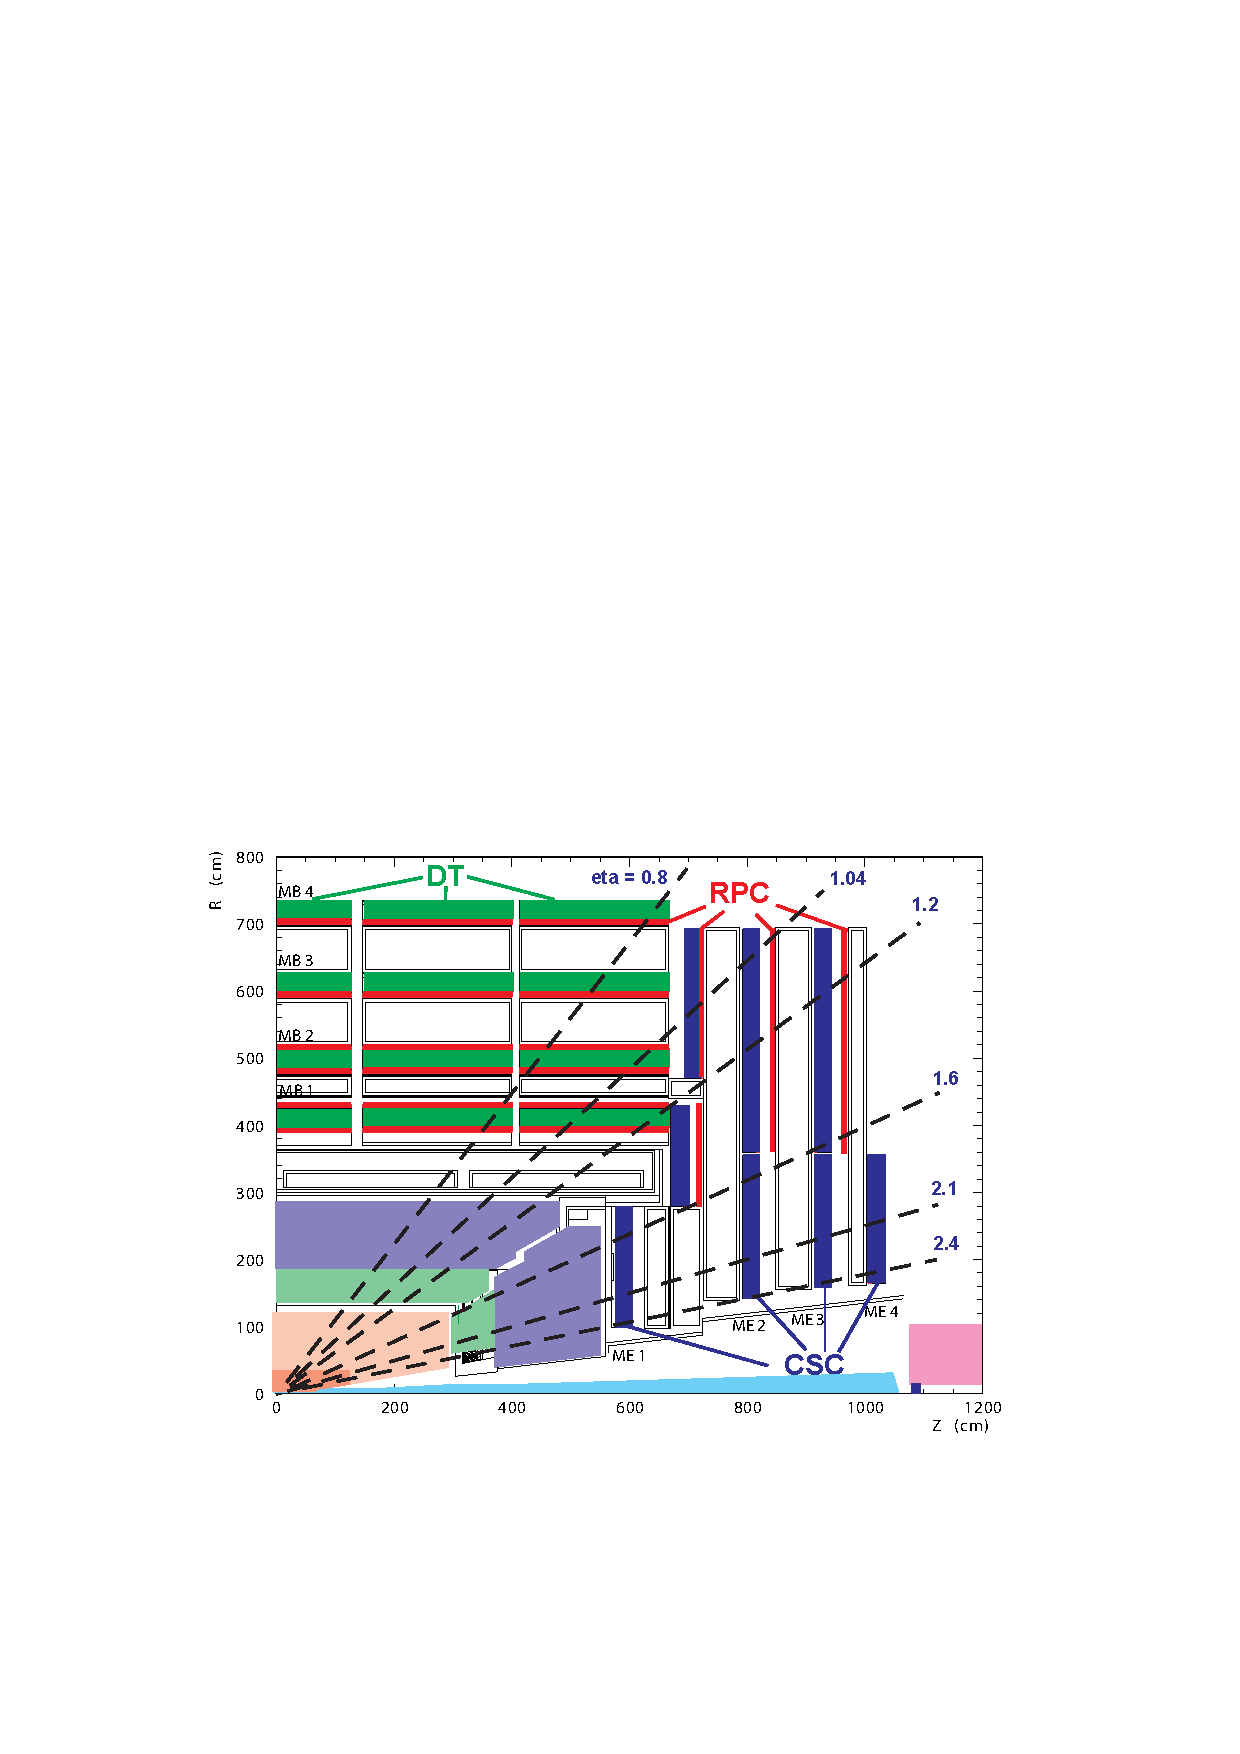
\includegraphics[width=0.9\textwidth]{figures/cms_muon}\hfil
\caption{Sketch of the CMS muon detectors. }
\label{fig:cms_muon}
\end{figure*}


In the barrel, the muon system is organized in chambers divided into 4 layers at radii of approximately 4.0, 4.9, 5.9 and 7.0 m from the beam axis. 
The layers are organized in 5 wheels along the beam axis, covering in total the region $|\eta| < 1.2$, and each wheel is divided into 12 stations, with each covering a $30^{o}$ azimuthal angle. 
Chambers in different stations are organized so that a high-p$_T$ muon produced near a sector boundary crosses at least 3 out of the 4 stations in each layer. 
Each station is designed to give a muon vector in space, with a $\phi$ precision better than 100 $\mu$m in position and approximately 1 mrad in direction. 
In the two innermost layers, each DT chamber is coupled between two RPCs, while, in the two outermost layers, each chamber is coupled to one RPC.

In each of the endcaps, the CSCs and RPCs are arranged in 4 disks perpendicular to the beam, and in concentric rings, 3 rings in the innermost station, and 2 in the others, totaling in 486 CSC chambers for both endcaps. 
The chambers are trapezoidal and cover either 10$^{o}$ or 20$^{o}$ in $\phi$. 
A muon in the pseudorapidity range $1.2 < |\eta | < 2.4$ crosses 3 or 4 CSCs. 
In the endcap-barrel overlap range, $0.9 < |\eta | < 1.2$, muons are detected by both the barrel DTs and endcap CSCs. 
The spatial resolution provided by each chamber from the CSCs is typically about 200 $\mu$m (100 $\mu$m for the innermost layer). The angular resolution in $\phi$ is of the order of 10 mrad.

\subsection{Luminosity Detectors}

The instantaneous luminosity is a key element to perform physics analysis at colliders in order to estimate how many events a certain process will yield given its cross section. 
The CMS experiment uses five different detectors to monitor and measure the instantaneous luminosity, based on different occupancy measurements for each individual detector. 
The used subdetectors are: the barrel DTs, the HF, the Pixel Luminosity Telescope (PLT) and the Fast Beam Condtions Monitor (BCM1f). 
The last two detectors use silicon pixel sensors and single-crystal diamonds, respectively, located close to the LHC beam pipe. 

These luminosity measurements are calibrated with dedicated LHC runs called Van der Meer (VdM) scans. 
By scanning the two beams through one another in the transverse plane of the detector, VdM scans allow to measure the luminosity per colliding bunch pair from machine parameters. 

\subsection{The CMS Trigger and Data Acquisition Systems}

The LHC provides bunch crossings with intervals of 25ns, which means that CMS produces collisions data at a rate of 40 MHz. 
The average event size produced by the CMS data acquisition system is of about 1 MB, which means that, if the experiment were to read and save every collision, it would need a data output bandwidth of approximately 40 TB/s. 
Such amount of data cannot be processed and saved by the current capabilities of the computing farms responsible for these tasks. 
However, most of these events are not of interest for the experiment: they consist of low energy QCD processes which would not be selected, in general, by any physics analysis. 
For this reason, CMS uses a trigger system that filters the collision data online. 
In general terms, the CMS trigger system must ensure a large acceptance for physics signals, while keeping the output rate and CPU time under control.

The first layer of the CMS trigger system is called the Level-1 (L1) trigger, and reduces the event rate from 40 MHz to 100 kHz. 
It works at hardware level, based on FPGA and custom ASIC integrated circuits technology, using information from the calorimeters and muon detectors to select, in about 4 $\mu$s, the most interesting events. 

The L1 is divided into three parts: the calorimeter trigger, the muon trigger and the global trigger.
The calorimeter trigger is itself divided into two steps: Layer-1 and Layer-2. 
In the first, it receives summarized data from the ECAL and HCAL in small packets called trigger primitives and computes basic information such as the sum of ECAL and HCAL energies and energy calibration as well as the computation of the H/E ratio (used to discriminate electrons and photon from hadronic jets). 
The information calculated by the Layer-1 is parallelized: each Layer-1 processor calculates local information pertaining to a section of the detector. 
The following step, the Layer-2 calorimeter trigger, receives the information from the Layer-1 and calculates global variables (such as total energy sum and calorimeter based missing transverse energy) and reconstructs simple versions of jets, taus and electrons/photons. 

The muon trigger receives information from the three muon subdetectors to ensure good coverage and redundancy. 
For the DTs and CSCs, the front-end trigger electronics identifies track segments from the hit information registered in multiple detector planes of a single measurement station, which are transmitted via optical fibers to regional track finder processors. 
These processors apply pattern recognition algorithms to identify muon candidates and measure their momenta from their bending under the CMS magnet. 
The combined muon trigger provides to the global trigger the transverse momentum of the muon candidates, along with their positions and quality scores, so they can be accepted/discarded by the global trigger. 

The global trigger, the final L1 step, is responsible for selecting interesting events based on the global information received from the Layer-2 calorimeter trigger and the last step of the muon trigger. 
These decisions are taken based on L1 selection algorithms stored in the electronics. 
This decision is informed to the central CMS data acquisition system, which transmits the full event data to processors that will format the data for the next trigger step, the High Level Trigger (HLT). 

The HLT is the final online selection step at CMS, and reduces the event rate from 100 kHz (L1 output) to a sustainable level of 1 kHz. 
It is implemented in software running on a farm of commercial computers which includes about 16,000 CPU cores. 
The HLT runs a simplified version of the full CMS object reconstruction, detailed below, based on the CMS software architecture CMSSW, optimized for the CPU timing requirements that exist at trigger level. 


\subsection{Object Reconstruction at CMS}

The general object reconstruction at CMS can be summarized in Figure \ref{fig:cms_reco}. 
It takes advantage of the CMS geometry, the cylindrical onion, and gathers information from different subdetectors to reconstruct a single type of particle: charged hadrons will leave hits in the tracker and will be stopped by the HCAL; neutral hadrons will not leave hits in the tracker but will deposit their energy on the HCAL; electrons and photons will both deposit their energies on the ECAL, while the former will also leave hits in the tracker; muons will leave hits in the tracker and the muon system, with no energy deposits in the calorimeters. 
This global event description, which links information from the different subdetectors, is usually referenced as particle flow algorithms (PF) \cite{cms_pf}. 
The particles created with this event description are called PF candidates and are mutually exclusive. 
This means, for example, that a single track cannot be used to reconstruct two different PF candidates.
It's important to notice that using particle flow algorithms at CMS is only possible due to the high granularity and position resolution of all its parts, particularly its calorimeters. 

\begin{figure*}[h]
\centering 
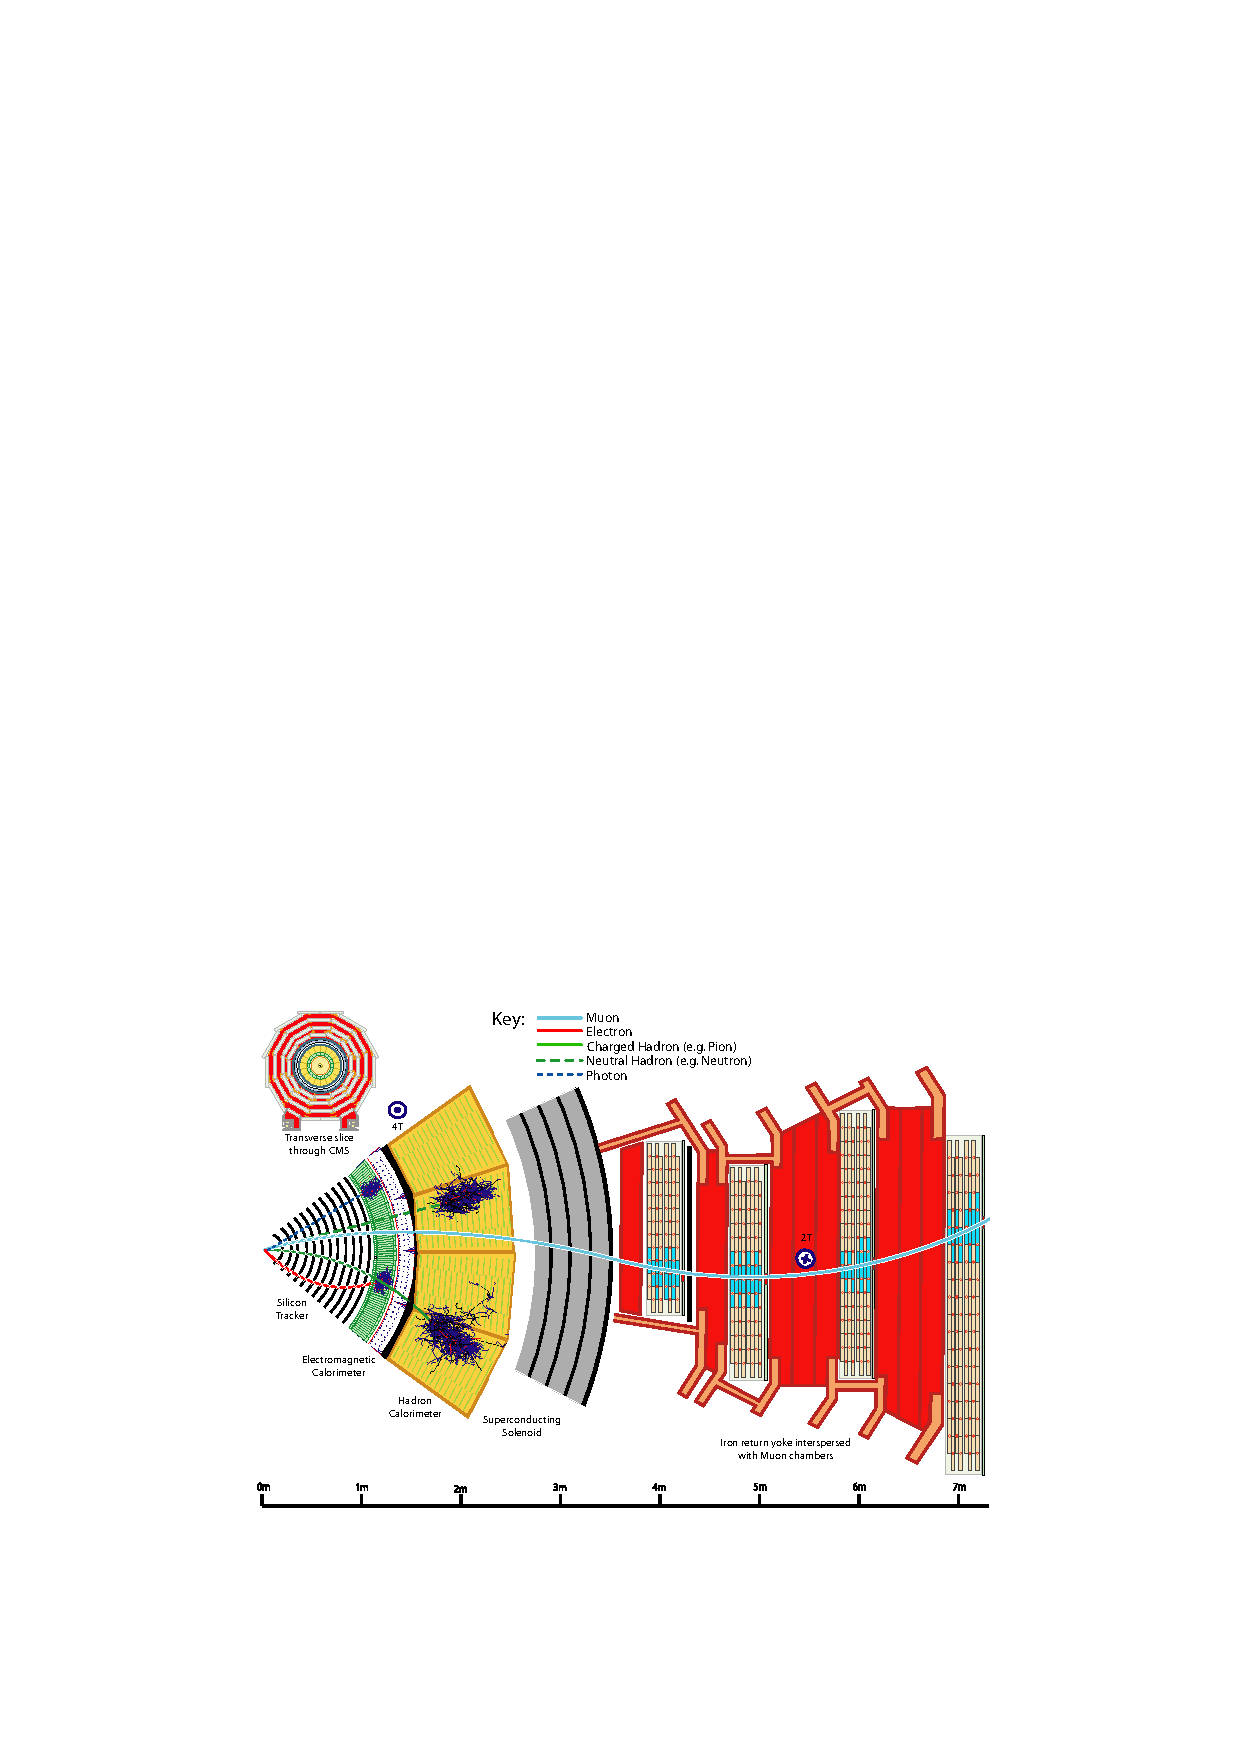
\includegraphics[width=0.9\textwidth]{figures/cms_reco}\hfil
\caption{Sketch of different types of object reconstruction at CMS. }
\label{fig:cms_reco}
\end{figure*}

The basic ingredients of the particle flow algorithm are the energy clusters on the calorimeters and the reconstructed trajectories obtained from the trackers and muon systems, which will be discussed below.  
Then, some of the objects reconstructed by CMS will be described, particularly the ones that are important in the analyses to be described in the following sections.

\subsubsection{Particle Flow Ingredients}

Tracks are the reconstructed trajectories of charged particles that leave hits in the CMS tracker \cite{cms_track}. 
Other than providing position information, these tracks are used to measure the particle's momentum via its bending under the CMS magnet. 
Track reconstruction starts with clusters of hits close to the beam pipe, in the inner pixel detector. 
Possible trajectories are then extrapolated and, if hits in the following tracker layers are found, they are added to the track and the track parameters are updated. 
After the algorithm hits the final tracker layers, and a first version of the full trajectory is reconstructed, another track reconstruction is performed, this time outside-in. 
The final track parameters are set to the weighted average of inside-out and outside-in results. 
The tracks have to fulfill quality criteria and are otherwise discarded. 
Finally, the used tracker hits are removed from the hit collection, and the procedure is repeated.

Primary vertices, which represent the point where a hard scatter event occurred during a bunch crossing, are reconstructed based on track clustering at the interaction region \cite{cms_track}. 
This region is at the center of CMS and has a typical length of $\approx$ 5-6 cm in the z direction, while its transverse dimension is $\approx$ 20-30 $\mu$m. 
Many primary vertices can be reconstructed for one bunch crossing. 
During the 2016 data taking period, events with over 50 primary vertices have been recorded by CMS. 
It is common to refer to the number of reconstructed primary vertices as "pile-up".

The fitting procedure used to extrapolate the tracks in the usual reconstruction does not perform well for electron tracks \cite{cms_track}. 
This happens because of the high amount of bremsstrahlung radiation electrons emit in the tracker, changing considerably the expected shape of their trajectory, which is not modeled by the standard algorithm. 
The electron-like tracks, selected based on their original fit quality and number of hits, are then refitted with a more appropriate method, the Gaussian-sum Filter (GSF), which allows for substantial non-Guassian energy loss along the trajectory.

Calorimeter clusters are reconstructed to detect and measure the energy of photons, electrons and hadrons, being the only source of measurement for photons and neutral hadrons \cite{cms_pf}. 
The clustering algorithm, that gathers in groups calorimeter deposits, is applied separately for the different calorimeter partitions: ECAL barrel, ECAL endcaps, HCAL barrel, HCAL endcaps, and each of the two preshower layers. 

The clustering procedure starts by searching for cluster seeds, which are local calorimeter-cell energy maxima, with respect to either its closest 8 or 4 cells, above a certain threshold. 
Topological clusters are grown from cluster seeds by adding together nearby seeds that share calorimeter cells. 
These topological clusters are used to estimate the energy sharing between clusters reconstructed from two different but nearby cluster seeds. 
Each individual cluster position is calculated as $X=\sum_{i}(w_{i}X_{i})/(\sum_{i}w_{i})$, with $w_{i}=ln(E_{i}/E_{th})$, where $E_{th}$ is an energy threshold and the $i$ is summed over the cells within a cluster.

\subsubsection{Photons and Electrons}

Electrons are reconstructed based on seed electron tracks reconstructed with the GSF algorithm. 
After a good quality electron track is found, it must be linked to an energy cluster on the ECAL. 
Photons, on the other hand, rely solely on the ECAL clusters to be reconstructed, since they leave no signal on the trackers. 
The reconstruction algorithm for ECAL clusters, called supercluster algorithm, allows almost complete recovery of the energy of photons that convert due to the material in front of the ECAL \cite{cms_egamma}. 
The corrections and calibrations involved to ensure a precise energy reconstruction for these particles will be described in the chapter dedicated to the CMS ECAL. 

Photons and electrons are identified based on a set of shower shape and isolation variables. 
The former measures the shape of the energy deposit on the ECAL, while the latter gives information about the event content surrounding the photon candidate. 
Isolation variables are particularly important when dealing with $\pi^{0}$ mesons, produced in hadronic showers, that decay to two almost colinear photons. 
These $\pi^{0}\rightarrow\gamma\gamma$ objects from jets must be filtered out of the photons collection in a physics analysis looking for photons coming from the hard scatter interaction. 
Shower shape variables also help to distinguish between between real photons and jets, but also give important information against non-collision backgrounds reconstructed as photons. 

For the ECAL, electron and photon clusters look approximately the same, therefore, almost indistinguishable when using only calorimeter information. 
In order to separate electrons from the photon collection, one must veto on possible tracks appearing within the photon cone. 
This is done in two different ways in CMS: via a conversion-safe electron veto, which vetos on electron tracks that are not compatible with photon conversion tracks, and via the pixel seed veto, which vetos on hits in the innermost layers of the pixel detector assuming the photon cone coming from a certain primary vertex.

\subsubsection{Jets}

As mentioned above, colored particles cannot be observed in a color non-neutral state. 
Therefore, we can only access the information (such as kinematics) about a quark/gluon in the final state experimentally through its hadronization product, the jets. 
The process of obtaining a jet from a quark or a gluon, however, cannot be modeled by perturbative QCD calculations, making it susceptible to many theoretical uncertainties and causing a "jet" to be ill-defined theoretically. 
There are, however, methods of jet reconstruction that minimize those uncertainties. 

The anti-$k_t$ and the Cambridge-Aachen (CA) methods are currently used by CMS and provide a jet reconstruction that are both infrared safe (avoiding low energy non-perturbative singularities) and colinear safe (avoiding singularities due to radiation colinear to the hadronizing particle) \cite{cms_jet}. 
Both algorithms work by combining PF candidates sequentially in a jet if a certain distance discriminant is smaller than a certain parameter. 
The analyses documented in this document use the anti-$k_t$ algorithm with a distance parameter $R=0.4$, as most analyses using the CMS Run 2 dataset.

The energy of the reconstructed jets must be corrected in order to match a jets produced with particles generated from a full Monte Carlo simulation of a hadronization process. 
This mismatch is attributed to the nonuniform and nonlinear response of the CMS calorimeters, electronics noise and pile-up. 
To correct for this, jet energy correction (JEC) factors are derived centrally by the CMS collaboration to be used by individual analyses. 
These JEC factors correct the (raw) 4-momenta parameters of the reconstructed jet as a multiplicative factor.

An important contributor to performance degradation in jet energy measurement is the pile-up. 
Extra charged hadrons from softer primary vertices can be erroneously clustered within the jet and bias the energy reconstruction. 
Therefore, a pile-up subtraction method that is called Charged Hadron Subtraction (CHS) is used in CMS. 
This is a particle-by-particle method that makes use of PF jets and exploits the excellent CMS tracking capabilities to identify and remove charged hadrons inside jets that are known to originate from pile-up vertices.

\subsubsection{Identification of b-quark jets}

Many interesting phenomena that are searched at the LHC involve bottom quarks. 
One important example is the $H\rightarrow b\bar{b}$ process, which has the highest branching fraction among the SM Higgs decays. 
Another example is the top quark decay, which is almost always to a bottom quark plus a W boson. 
These searches would be facing an enormous amount of background events if jets from bottom quarks were indistinguishable from lighter quark jets, copiously produced by the LHC. 
However, bottom quark jets (from now on simply referred to as b-jets) are strikingly different from their lighter counterparts due to the presence of a B meson (product of the bottom quark hadronization). 

B mesons can only decay via the weak interaction via Cabbibo suppressed processes $b\rightarrow Wc$ and $b\rightarrow Wu$. 
This causes the average lifetime of a B meson to be of about 1.5 picoseconds. 
Assuming they are produced at the speed of light, these mesons can travel around 0.5 milimeters before decaying. 
This decay length is well within the reach of the current CMS tracking resolution, therefore, the vertex of the B meson decay (secondary vertex) can be measured. 
With this information, algorithms (b-taggers) can be constructed to distinguish b-jets from light jets.

The b-tagger algorithm utilized in the analyses presented in this thesis is the Combined Secondary Vertex (CSV) algorithm \cite{cms_btag}. 
This method uses multiple reconstruction quantities related to the tracks associated to the jet constituents and the properties of secondary vertices reconstructed inside the jet, if present. 
The CSV algorithm is still applicable, however, when no secondary vertices are associated to the jet. 
The variables used by this method include the number of tracks in the jet, the significance of the tracks impact parameters, and, if available, the impact parameter, mass and number of tracks associated to the secondary vertex. 
These variables are used to determine a single likelihood discriminator associated to the jet, i.e. the CSV discriminator, proportional to the compatibility of the jet with a b-quark decay.













